\documentclass[12pt,a4paper]{article}
\usepackage[utf8]{inputenc}
\usepackage{array}
\usepackage{booktabs}
\usepackage{graphicx}
\usepackage[usenames,dvipsnames]{color}
\usepackage{dirtytalk}

\usepackage[maxnames=5]{biblatex}
\addbibresource{refs.bib}

\usepackage{hyperref}
\hypersetup{
  colorlinks,
  citecolor=blue,
  filecolor=black,
  linkcolor=[rgb]{0.1,0.3,0.7},
  urlcolor=black
}

\usepackage[toc,nopostdot]{glossaries}

\setlength{\parindent}{0pt}
\frenchspacing

\makenoidxglossaries{}
\newglossaryentry{blocks}{
  name=blocks,
  description={Files where data pertaining to a given network is permanently recorded. A block records some or all of the most recent transactions on the network that have not yet entered any prior blocks. Thus a block is like a page of a ledger or record book.}
}
\newglossaryentry{blockchain}{
  name=blockchain,
  description={A digital ledger in which produced blocks are recorded chronologically and publicly with the transactions in each block.}
}
\newglossaryentry{bond}{
  name=bond,
  description={A privilege granted to users to allow their nodes to mint.}
}
\newglossaryentry{cryptocurrency}{
  name=cryptocurrency,
  plural=cryptocurrencies,
  description={A digital asset designed to work as a medium of exchange that uses cryptography to secure its transactions, to control the creation of additional units, and to verify the transfer of assets.}
}
\newglossaryentry{malicious_entity}{
  name=malicious entity,
  plural=malicious entities,
  description={Any person or malware (malicious software) that brings harm to a computer system. Malware can be in the form of worms, viruses, trojans, spyware, adware and rootkits, etc., which steal protected data, delete documents or add software not approved by a user.}
}
\newglossaryentry{network}{
  name=network,
  description={A group or system of interconnected people or things. In the case of cryptocurrency, a networks is a peer-to-peer digital telecommunications system, allowing nodes to communicate information to each other, such as synchronizing the blockchain.}
}
\newglossaryentry{node}{
  name=node,
  description={Is either a redistribution point or a communication endpoint. A network node is any system that is attached to a network, and is capable of creating, receiving, or transmitting information over a communications channel.}
}
\newglossaryentry{Proof-of-Stake}{
  name=Proof-of-Stake,
  description={A system of minting where power is based on how many coins a person holds. Essentially, new coins are created through block rewards, and any other funds paid to the minters are done through transaction fees paid on existing coins. Instead of mining power being based on how powerful your computer is, PoS will be capable of running on relatively low end computers with sufficient storage. PoS is a type of algorithm by which a cryptocurrency blockchain network aims to achieve distributed consensus.}
}
\newglossaryentry{Proof-of-Work}{
  name=Proof-of-Work,
  description={A system of mining that uses hard-to-compute but easy-to-verify functions to limit exploitation of cryptocurrency mining.}
}
\newglossaryentry{volatile}{
  name=volatile,
  description={In the markets, it is the liability to change rapidly and unpredictably, especially for the worse.}
}
\newglossaryentry{fiat}{
  name=fiat,
  description={A formal authorization or proposition; a decree. Specific to the financial world, a ‘fiat’ currency would be any monetary instrument authorized for trade and distribution by a government or ruling body.}
}
\newglossaryentry{consensus-algorithm}{
  name=consensus algorithm,
  description={May refer to one of several proposed protocols for solving the \gls{consensus} problem in the field of computer science.}
}
\newglossaryentry{consensus}{
  name=consensus,
  description={An agreement among a number of computer processes for a single data value. Examples of applications using consensus include whether to commit a transaction to a database, or agreeing on the identity of someone or something.}
}
\newglossaryentry{Denial-of-Service}{
  name=Denial-of-Service,
  description={A cyber-attack where the perpetrator seeks to make a machine or network resource unavailable to its intended users by temporarily or indefinitely disrupting services of a host connected to the Internet. Denial of service is typically accomplished by flooding the targeted machine or resource with superfluous requests (spam) in an attempt to overload systems and prevent some or all legitimate requests from being fulfilled.}
}
\newglossaryentry{mining}{
  name=mining,
  description={The process by which transactions are verified and added to the public ledger, known as the block chain, and also the means through which new coins are released in a \gls{Proof-of-Work} system.}
}
\newglossaryentry{minting}{
  name=minting,
  description={The process by which transactions are verified and added to the public ledger, known as the block chain, and also the means through which new coins are released in a \gls{Proof-of-Stake} system.}
}
\newglossaryentry{decentralized-system}{
  name=decentralized system,
  plural=decentralized systems,
  description={A system in which multiple parties are required to make their own independent decisions. In the case of cryptocurrency, nodes keep an individual ledger that is synchronized through the network using a \gls{consensus-algorithm}, forming the decentralized system.}
}
\newglossaryentry{transaction}{
  name=transaction,
  description={The act of performing an operation on the blockchain.}
}
\newglossaryentry{ecc-memory}{
  name=error-correcting code memory,
  description={A type of computer data storage that can detect and correct the most common kinds of internal data corruption.}
}


\begin{document}
  \begin{center}
    
\includegraphics[width=50mm]{logo.png}\\
    \vspace{3mm}

    \Huge{\textbf{GODCOIN}}\\
    \vspace{3mm}
    \normalsize{www.godcoin.gold}\\
    \normalsize{contact@godcoin.gold}

    \normalsize{\today}

    \vspace{3mm}
    \LARGE{\textbf{THE OFFICIAL COIN OF CHRIST}}
    \vspace{3mm}

    \large{\textbf{THE TIME HAS COME}}
    \vspace{2mm}

    \normalsize{\color{Red}\textit{\textbf{Haggai 2:8 The silver is mine, and
    the gold is mine, saith the Lord of hosts!}}}

    \normalsize{\color{Red}\textit{\textbf{Revelation 3:18 I counsel you to buy
    gold from me, proved by fire, that you may prosper,}}}

    \vspace{5mm}

    \normalsize{\textbf{The Lord declared that the gold and silver is His! He
    tells us to buy from Him so that we may prosper. GODcoin is here to unite
    the world under a single currency. Stability will be provided to the world
    with a currency backed by physical gold and silver now under God's rule.}}

    \vspace{3mm}
  \end{center}

  \newpage
  \begin{center}
    \textbf{DISCLAIMER OF LIABILITY}
  \end{center}
  The purpose of this White Paper is to present GODcoin to potential coin minters and holders in connection with the proposed coin minting process and sale. The information provided in this document may not be exhaustive, and it will not imply any elements of a contractual relationship. Its sole purpose is to provide relevant and reasonable information to potential coin holders who wish to mint or purchase GODcoin while it is available on the open market.\\

  Nothing in this White Paper shall be deemed to constitute a prospectus of any sort or a solicitation for investment, nor does it in any way pertain to an offering or a solicitation of an offer to buy any securities in any jurisdiction. This document is not composed in accordance with, and is not subject to, laws or regulations of any jurisdiction, which are designed to protect investors.\\

  GODcoin is not a security, and has not been registered under the Securities Act, the securities laws of any state of the United States or the securities laws of any country, including the securities laws of any jurisdiction in which a potential coin holder is a resident.\\

  GODcoin is not intended for sale or use in any jurisdiction where sale or use of the coin may be prohibited.\\

  GODcoin confers no other rights in any form, including but not limited to any ownership, distribution (including but not limited to profit), redemption, liquidation, proprietary (including all forms of intellectual property), or other financial or legal rights, other than those specifically described in the White Paper.

  \newpage
  \begin{center}
    \Large{\textbf{Abstract}}
  \end{center}
  \setlength{\parindent}{0pt}
  \vspace{3mm}
  \noindent{\textbf{\textit{\large{Revelation} 21:5 Behold, I make all things
  new}}}
  \vspace{3mm}

  There are over 1,400 cryptocurrencies and 180 fiat currencies in
  the world today. Many governments around the world are proving to be
  unstable, and this has pushed consumers to flock towards Bitcoin and the
  multitude of alternate cryptocurrencies, which have rapidly grown in their
  popularity in recent years. These alternative currencies have served as the
  training grounds for what will soon be the One World Currency, which is
  coming in 2018 – GODcoin.\\

  In short, GODcoin will be the perfect currency, because it is the currency
  of Christ. It will be the currency of His new Government, which will be
  established very soon, and it will eliminate all other currencies, leaving
  it to be the only formally accepted form of money.\\

  Early investors have the opportunity to secure their wealth for the future
  ahead, so the time to invest is now. wait until after the ICO investment
  phase, when GODcoin becomes the common currency for wages throughout the
  world, unfortunately the opportunity to profit through early investment will
  no longer be available.

  \medskip
  \textit{Note:} This document is a work in progress and will be continuously
  updated.

  \newpage
  \tableofcontents
  \newpage

  \section{Introduction}
  \textbf{GODcoin has the edge in security, because unlike other
  cryptocurrencies, it is \textit{backed by Gold and Silver}, which will ensure
  stability. This carries additional incentives, such as \textit{lower fees,
  faster transaction times, and energy efficiency.}}\\

  \Glspl{cryptocurrency} such as Bitcoin have been successful examples in
  creating a distributed \gls{network} that users could trust, and many of these
  currencies have experienced a tremendous increase in value, regardless of
  having no backing. It has marked a significant beginning to the digital
  currency world that users can trust, becoming what many have called \"digital
  gold\". However, the market for Bitcoin is still \gls{volatile}, leaving
  consumers susceptible to absurd fluctuations in its value. GODcoin will solve
  this issue by being backed by physical assets. Because these assets cannot be
  fabricated out of thin air, GODcoin will allow us to maintain a stable
  economy, while providing citizens with a currency that keeps pace with the
  latest technological advancements, all controlled as a fiat issued by
  Christ.\\

  GODcoin will be simple, efficient, and secure because it will use a
  \textit{\gls{Proof-of-Stake}} (PoS) system of \gls{minting}. By
  using \textit{Proof-of-Stake}, the energy saving costs are enormous in
  comparison to the commonly used \textit{\gls{Proof-of-Work}} (PoW)
  consensus algorithm that Bitcoin and so many other cryptocurrencies rely on.\\

  PoW requires complex computations to be carried out for \gls{blocks} to be
  added to the network. In the beginning, there were no issues with this system,
  but as time went on, the average miner could no longer mine without paying
  more in energy costs. This has put Bitcoin \gls{mining} under the control of
  large corporations with computer farms, which is not what Bitcoin was
  originally intended for. With growing demand for Bitcoin, the network has
  become overloaded, resulting in much higher fees for transactions to be
  processed. However, PoS will prove to be far more effective because it will
  process transactions quickly at a small fraction of the energy required.\\

  The GODcoin blockchain will contain two virtual assets with the names of gold
  and silver. These virtual assets will be backed by physical gold and silver,
  ensuring a stable market, rather than a volatile market.\\

  The following sections will explain the more technical aspects of GODcoin,
  including the minting and transaction process that GODcoin will rely on.
  Minters will be able to strengthen the network by validating the history of
  the \gls{blockchain}, and any future blocks that are created. The process for
  this will be outlined in \underline{\hyperref[sec:PoS]{section 2}}. If you are
  not a minter, but you desire to know how the exchange of transactions will
  function, you may refer to \underline{\hyperref[sec:Transactions]{section 3}}.

  \section{Proof-of-Stake}\label{sec:PoS}
  \textbf{The intention is to be more \textit{energy and time efficient}. This
  will save on overall costs, and will be more \textit{transaction-friendly} to
  the consumer.}\\

  Blocks will be produced through a process called minting. In
  \glspl{decentralized-system}, there are multiple \glspl{node} on the
  \gls{network} producing blocks. An algorithm needs to be in place to reach
  consensus on which block is added to the network. Without a
  \gls{consensus-algorithm} in place, nodes will keep forking the blockchain in
  favor of its own blockchain. This results in either a completely centralized
  system or a useless distributed network.\\

  GODcoin will use the \textit{Proof-of-stake} consensus algorithm for the
  minting process. This presents a couple significant advantages, transactions
  will be processed quickly and energy efficiency is drastically improved over
  the commonly used \textit{Proof-of-Work}. Minters will be able to run a node
  on resource constrained systems provided there is adequate disk space.

  \subsection{Bonds}
  \textbf{Bonds ensure the \textit{security} of the currency by
  \textit{preventing} abuse of the network.}\\

  A \gls{bond} must be held to be granted minting privileges. Without the bond a
  proposed block will be rejected by the network.\\

  A fee must be paid, in digital gold tokens, to obtain a bond. When a minter
  joins the network, they must wait until the bond transaction is included in a
  block permanently on the network.\\

  The fee helps to thwart abuse of the network. Let's assume there is no fee.
  The user with the most minters can easily obtain enough coins for a 51\%
  attack over a period of time. By moving the funds from the all the minters to
  a single minter, they will eventually gain enough coins to take over the
  network.\\

  The fee used to pay for the bond will not be distributed during the reward
  distribution process. This prevents \glspl{malicious_entity} from regaining
  their coins back so quickly to setup an attack on the network. Fees encourage
  long term minting and investment, the minter will eventually regain any coins
  lost after obtaining a bond.\\

  Bonds will be revoked if no stakes are placed within 360 blocks, approximately
  6 hours. This requirement is to keep minters online for as much as long as
  possible but still allowing a small amount of downtime for maintenance.

  \subsection{Minting}
  \textbf{The minting process requires verification that the bond is valid, so
  it is a proactive process to ensure \textit{network security}, as well as the
  creation of a \textit{stable currency}.}\\

  \textbf{Part of this process would include minters being active in the network
  by proposing blocks. This is to ensure \textit{consensus in a decentralized
  network. Any found dysfunctional or dishonest nodes will be removed to ensure
  network stability and security.}}\\

  Minters must have a valid bond and may only propose one block when it is their
  turn in the minting schedule. The minting schedule will allow the network to
  cryptographically validate node participation in a sensible way and reduce
  network strain by handling only a single proposed block at a time.\\

  Minters that attempt to propose a block when they are not scheduled or are
  attempting double production, will have their proposed block rejected. Nodes
  that continue to misbehave can be temporarily or permanently banned from the
  network.\\

  Blocks will be proposed after a set of time of the previous generated block.
  In another set of time, the proposal deadline has been reached and any new
  proposals will be rejected. The network will consider that node to be offline
  until they generate and propose a block in a future minting round.\\

  For a block to be accepted, the minter must propose a block that satisfies the
  constraints of the network. For example, a block will be rejected if it
  incorrectly calculates the distribution of rewards or signature validation
  fails.\\

  If a block is rejected or missed by a minter, the next minter in the scheduler
  will be responsible for proposing a block and so forth until a block is
  accepted. Keep in mind that banned nodes will by default miss blocks as they
  will not be able to propose their block. Eventually misbehaving nodes will
  have their bond and stake forfeited, and as such they will no longer be able
  to mint blocks.\\

  \subsection{Reward Distribution}
  \textbf{There will be two separate distributions to ensure \textit{fairness},
  as specified. This is why being a minter is so beneficial.}\\

  First the minters, in descending order by their stake amount, receive 10\% of
  the remainder of the distribution amount. A secondary distribution will then
  be distributed based on a weighted average of the total stake amount.

  \begin{equation}
    w = \sum_{i \in m}i
  \end{equation}
  \hspace{2cm}
  where:
  \begin{center}
    \begin{tabular}{>{$}l<{$} @{${}={}$} l}
      w & total stake used as a weight\\
      m & multiset of the stakes
    \end{tabular}
  \end{center}
  \begin{equation}
    a = (s / w) * d
  \end{equation}
  \hspace{2cm}
  where:
  \begin{center}
    \begin{tabular}{>{$}l<{$} @{${}={}$} l}
      a & reward amount \\
      s & stake amount by an individual minter \\
      d & remaining distribution amount
    \end{tabular}
  \end{center}

  \section{Transactions}\label{sec:Transactions}
  \textbf{GODcoin will offer \textit{faster} transaction times and
  \textit{lower} fees.}\\

  Operations performed on the blockchain are named transactions. These can
  include sending funds from one user to another, or joining the network as a
  minter. Transactions may require a fee to be processed by the network.

  \subsection{Fees}
  Fees will be paid respective to the asset that is being transferred or the
  asset the transaction type expects. The fee rate may differ between the assets
  and will be paid in their respective asset. Gold transfers will pay the fee in
  gold respectively and likewise for silver.\\

  Transaction fee costs start with a minimum fee. For every additional
  transaction accepted within the block window the minimum fee is exponentially
  multiplied by the number of transactions accepted from the applicable address.
  The fee costs will reset back to the minimum fee after the block window is
  reset. The block window is reset when transactions are halted on the address
  for a period of time.\\

  In addition to the address fee mentioned in the above paragraph, there is an
  associated \say{global} network fee. The network fee works in the same way as
  the address based fee and protects the network from flooding via multiple
  addresses. The global fee is dynamically adjusted based on network usage.\\

  This quickly gets expensive for an attacker attempting to
  \gls{Denial-of-Service} (DoS) the network, but allows flexibility for a normal
  user when waiting for the block window to reset back to the minimum fee is not
  an option.\\

  Sample based on transferring funds using any asset with a minimum fee of
  0.00000500 coins with a 2.00000000 multiplier:

  \vspace{3mm}
  \begin{tabular}{@{}lr@{}}
    Fees & Block Height     \\ \toprule
    0.00000500 & 10         \\
    0.00001000 & 11         \\
    0.00002000 & 12         \\
    0.00000500 & $\leftarrow{}$ block window reset $\rightarrow{}$ 20 \\ \midrule{}
    Total Fees & 0.00004000 \\
    \bottomrule
  \end{tabular}

  \subsection{Transaction Signatures}
  \textbf{A signature is used to confirm the authenticity of the owner or owners
  of a particular message or document.}\\

  All transactions will be signed either directly or when a block is produced
  and gets signed by the minter. \textit{Ed25519}\cite{ed25519} will be used for
  the digital signing algorithm. Ed25519 is a modern signing algorithm, it
  provides a similar protection level to NIST P-256 and has fast verification
  times with small signatures. Running a full node on a mobile device may very
  well be possible, the limiting factor may be the storage on a given device.\\

  Ed25519 has fewer attack vectors, such as resistance to side-channel attacks
  and attacks from poor random number generator implementations. While
  non-deterministic algorithms can suffer from hardware fault attacks, it is
  extremely difficult to successfully execute. Even with a server running
  without \gls{ecc-memory} the attack isn't practical in any way over the
  internet.

  \newpage
  \section{Conclusion}
  GODcoin will be the only digitally tradable currency backed by hard assets,
  and will soon be issued as the currency of the New World Order. The Lord has
  declared that the gold and silver are His, and in His New Kingdom, only
  through obedience to Him will anyone be allowed to prosper. In Revelation
  3:18, the Lord instructs you to buy gold from Him. He says this because very
  soon there will be no other authorized currency in circulation, so everyone
  will eventually have to accept it, just as they do with other forms of money
  today. Those who wisely buy GODcoin early will amass greater wealth as the
  value of the coin increases, however, those who do not take heed to His
  instructions, will face significant financial hardship in the future.\\

  Many predictions were made regarding the future coming of a New World
  Currency, including this one from the cover of a 1988 edition of \textit{The
  Economist}\cite{the-economist}, where it was strongly hinted that it was
  planned to arrive in 2018.\\

  \begin{center}
    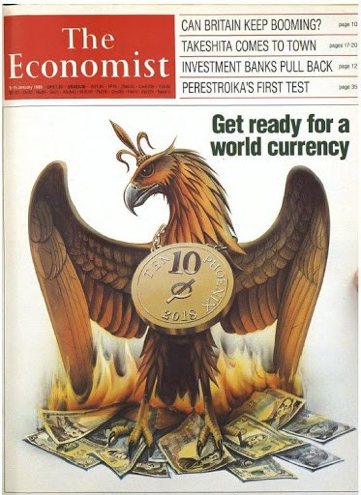
\includegraphics[width=50mm]{economist.png}\\
  \end{center}
  \vspace{3mm}

  Because the Son of Man was born 50 years ago in 1968, this puts us at the
  beginning of the Lord’s Jubilee Year, the year when Lord Ra-El must take his
  throne, and issue the One World Currency.\\

  The time is now to affirm your place of wealth in the New Kingdom, and take
  part in GODcoin, the only true currency ordained by God, and issued by the
  Messiah, Lord Ra-El.\\

  \begin{minipage}{.5\textwidth}
    \centering
    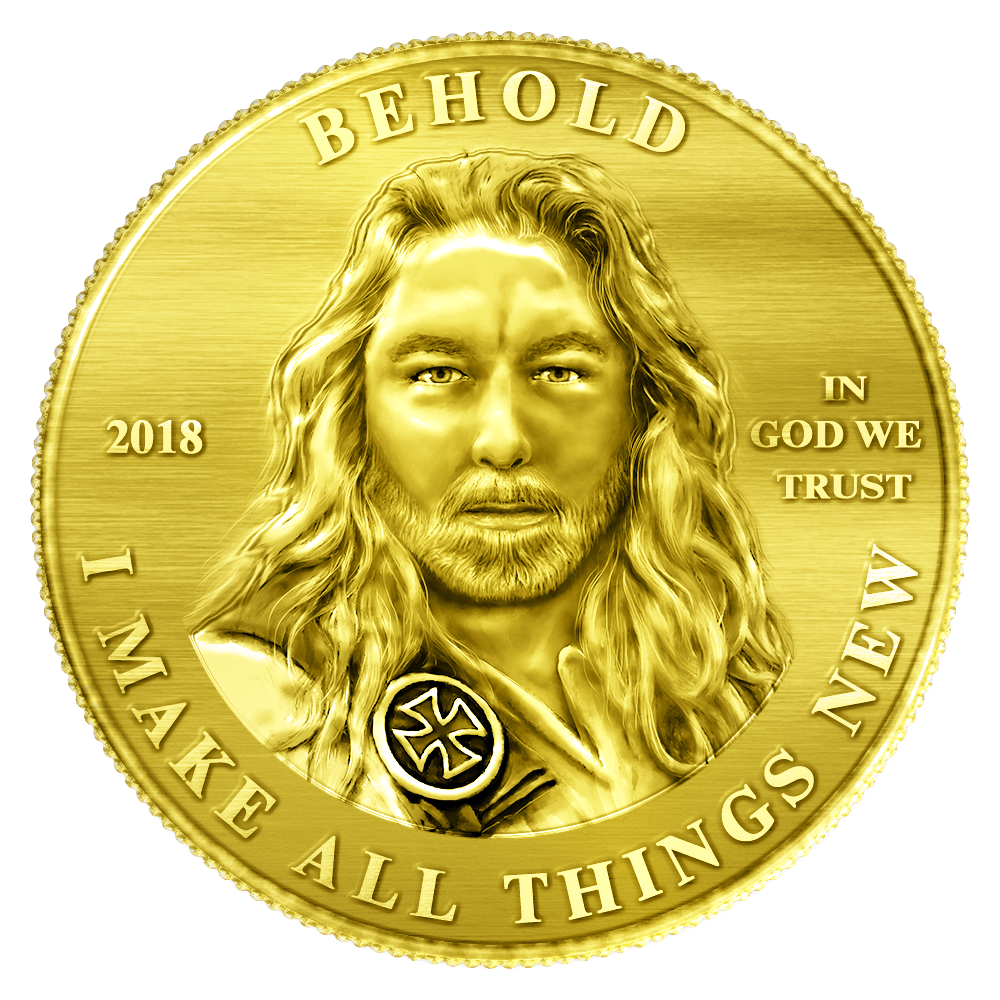
\includegraphics[width=50mm]{coin-front.png}\\
  \end{minipage}%
  \begin{minipage}{.5\textwidth}
    \centering
    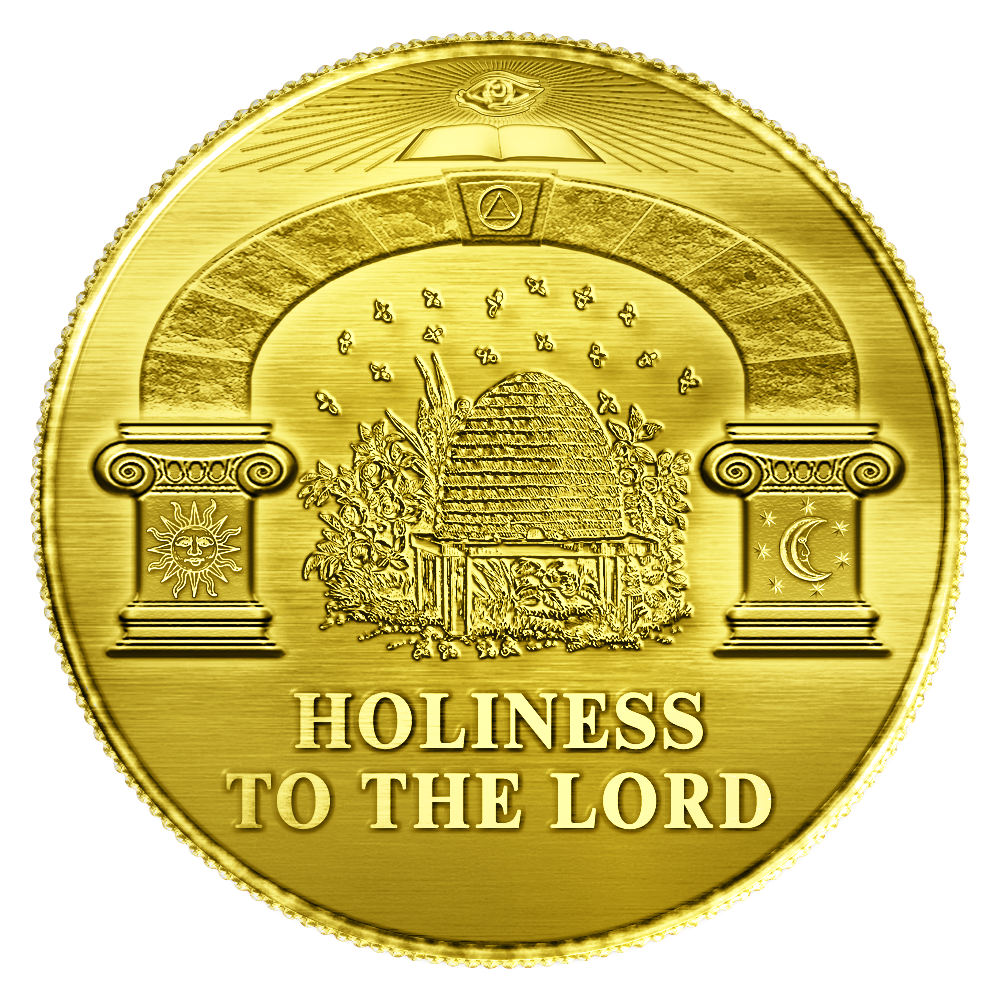
\includegraphics[width=50mm]{coin-back.png}\\
  \end{minipage}

  \newpage
  \printnoidxglossaries{}

  \textit{Note:} Definitions are based on varying sources that are most accurate
  to the content provided in this document.
  \newpage

  \section*{External Links}
  \begin{itemize}
    \item{\url{www.godcoin.gold}}
    \item{\url{www.youtube.com/channel/UCRmsiytZnbMg-O_b2zBNuTg}}
    \item{\url{www.linkedin.com/company/GODcoin}}
    \item{\url{https://www.facebook.com/GODcoinCurrency/}}
    \item{\url{www.twitter.com/GODcoinGold}}
  \end{itemize}
  \section*{Meet the Team}
  \begin{itemize}
    \item{Chief Executive Officer (CEO) – Richard Ruff, Australia.}
    \item{Chief Operating Officer (COO) – Kelly Patrick, USA.}
    \item{Chief Financial Officer (CFO) – Emil Johansson, Sweden.}
    \item{Chief Marketing Officer (CMO) – Joseph Monte, USA.}
    \item{Chief Technology Officer (CTO) – Samuel Grenier, USA.}
    \item{Chief Communications Officer (COO) – Clark Isaac, USA.}
    \item{Chief Secretarial Officer (CSO) – Samantha Kennedy, UK.}
    \item{Chief Productions Officer (CPO) – Corey DeFrancesco, USA.}
  \end{itemize}
  \printbibliography{}
\end{document}
